\documentclass[12pt, a4paper]{article}
\usepackage{ctex}

\usepackage{float}
\usepackage[super, square]{natbib}
\usepackage[margin = 1in]{geometry}
\usepackage{
  color,
  clrscode,
  amssymb,
  ntheorem,
  amsmath,
  listings,
  fontspec,
  xcolor,
  supertabular,
  multirow
}
\definecolor{bgGray}{RGB}{36, 36, 36}
\usepackage[
  colorlinks,
  linkcolor=bgGray,
  anchorcolor=blue,
  citecolor=black
]{hyperref}
\newfontfamily\courier{Courier}

\theoremstyle{margin}
\theorembodyfont{\normalfont}

\newtheorem{theorem}{Theorem}
\newtheorem{definition}[theorem]{Definition}
\newtheorem{example}[theorem]{Example}

\newcommand{\st}{\text{s.t.}}
\newcommand{\mn}{\mathnormal}
\newcommand{\tbf}{\textbf}
\newcommand{\fl}{\mathnormal{fl}}
\newcommand{\f}{\mathnormal{f}}
\newcommand{\g}{\mathnormal{g}}
\newcommand{\R}{\mathbf{R}}
\newcommand{\Q}{\mathbf{Q}}
\newcommand{\JD}{\textbf{D}}
\newcommand{\rd}{\mathrm{d}}
\newcommand{\str}{^*}
\newcommand{\vep}{\varepsilon}
\newcommand{\lhs}{\text{L.H.S}}
\newcommand{\rhs}{\text{R.H.S}}
\newcommand{\con}{\text{Const}}
\newcommand{\oneton}{1,\,2,\,\dots,\,n}
\newcommand{\aoneton}{a_1a_2\dots a_n}
\newcommand{\xoneton}{x_1,\,x_2,\,\dots,\,x_n}


\title{E06c 编程作业解答}
\author{姓名:范舟 \quad 学号:516030910574}
\date{}

\begin{document}
\lstset{numbers=left,
  basicstyle=\scriptsize\courier,
  numberstyle=\tiny\courier\color{red!89!green!36!blue!36},
  language=Matlab,
  breaklines=true,
  keywordstyle=\color{blue!70},commentstyle=\color{red!50!green!50!blue!50},
  morekeywords={},
  stringstyle=\color{purple},
  frame=shadowbox,
  rulesepcolor=\color{red!20!green!20!blue!20}
}
\maketitle

\paragraph{注意:} 
\begin{enumerate}
\item 程序在文档中也要粘贴,同时把代码和该文档放在同一个文件夹中打包发给我.(建议多个同学或整个班级一起打包;邮箱: terenceyuyue@sjtu.edu.cn)
\item 该文档不需打印,只收电子版.
\end{enumerate}

\paragraph{问题:} 用不同数值方法计算积分$\int_{0}^{1} \sqrt{x} \ln{x} \rd x = -\frac{4}{9}$.

\section{复化求积方法}
\paragraph{1.1} 编写复化梯形公式的函数文件,命名为Trapezoidal.m,画出最大模误差与步长$h$的函数图像.\\
注:计算中涉及到的求和可通过sum命令完成,避免循环.\\
下面是Trapezoidal函数的实现,其中参数f是被积函数的函数句柄,a与b为积分上下界,n为等分的小区间数目.
\lstinputlisting{./Ex6c-code/Trapezoidal.m}
下面的程序(test\_room.m)调用Trapezoidal函数计算题目中的积分,并计算步长$h$取不同值时的最大模误差,并画出图像.这段程序也用于调用后面编写的其他积分函数进行测试与绘图.
\lstinputlisting{./Ex6c-code/test_room.m}
\begin{figure}[H]
  \begin{center}
    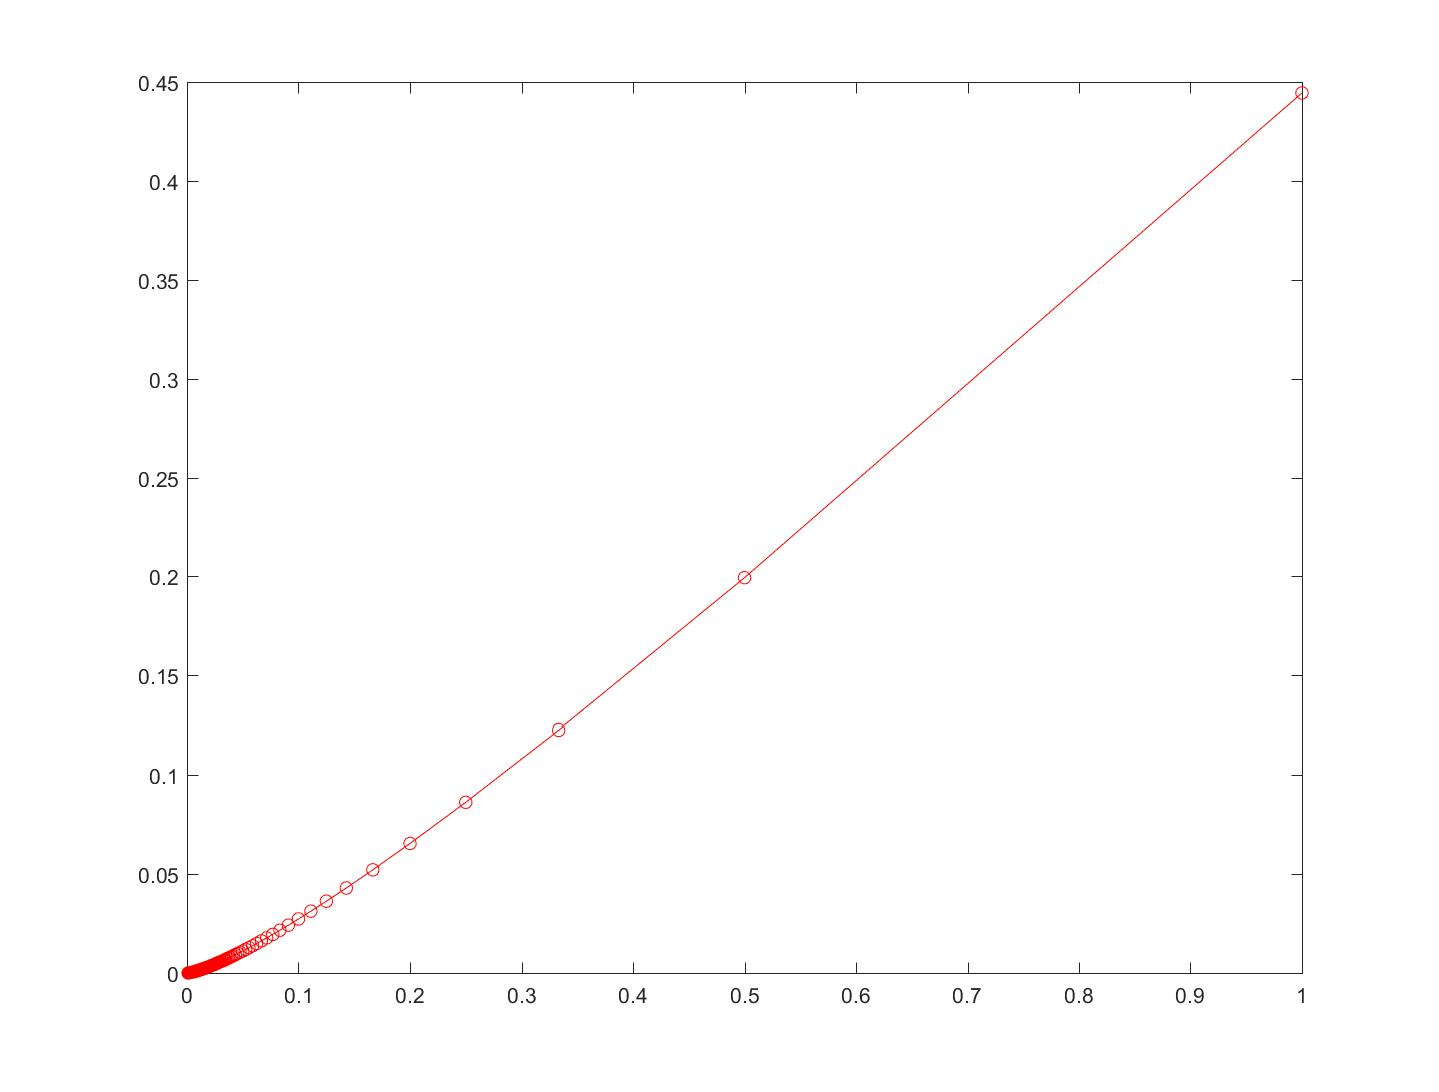
\includegraphics[height=12cm]{./Ex6c-code/trapezoidal.jpg}
    \caption{使用复化梯形公式的最大模误差与步长$h$的函数图像}
  \end{center}
\end{figure}
\paragraph{1.2} 编写复化Simpson公式的函数文件,命名为Simpson.m,画出最大模误差与步长$h$的函数图像.
\lstinputlisting{./Ex6c-code/Simpson.m}
使用test\_room.m调用Simpson函数计算题目中的积分,并计算步长$h$取不同值时的最大模误差,画出图像如下.
\begin{figure}[H]
  \begin{center}
    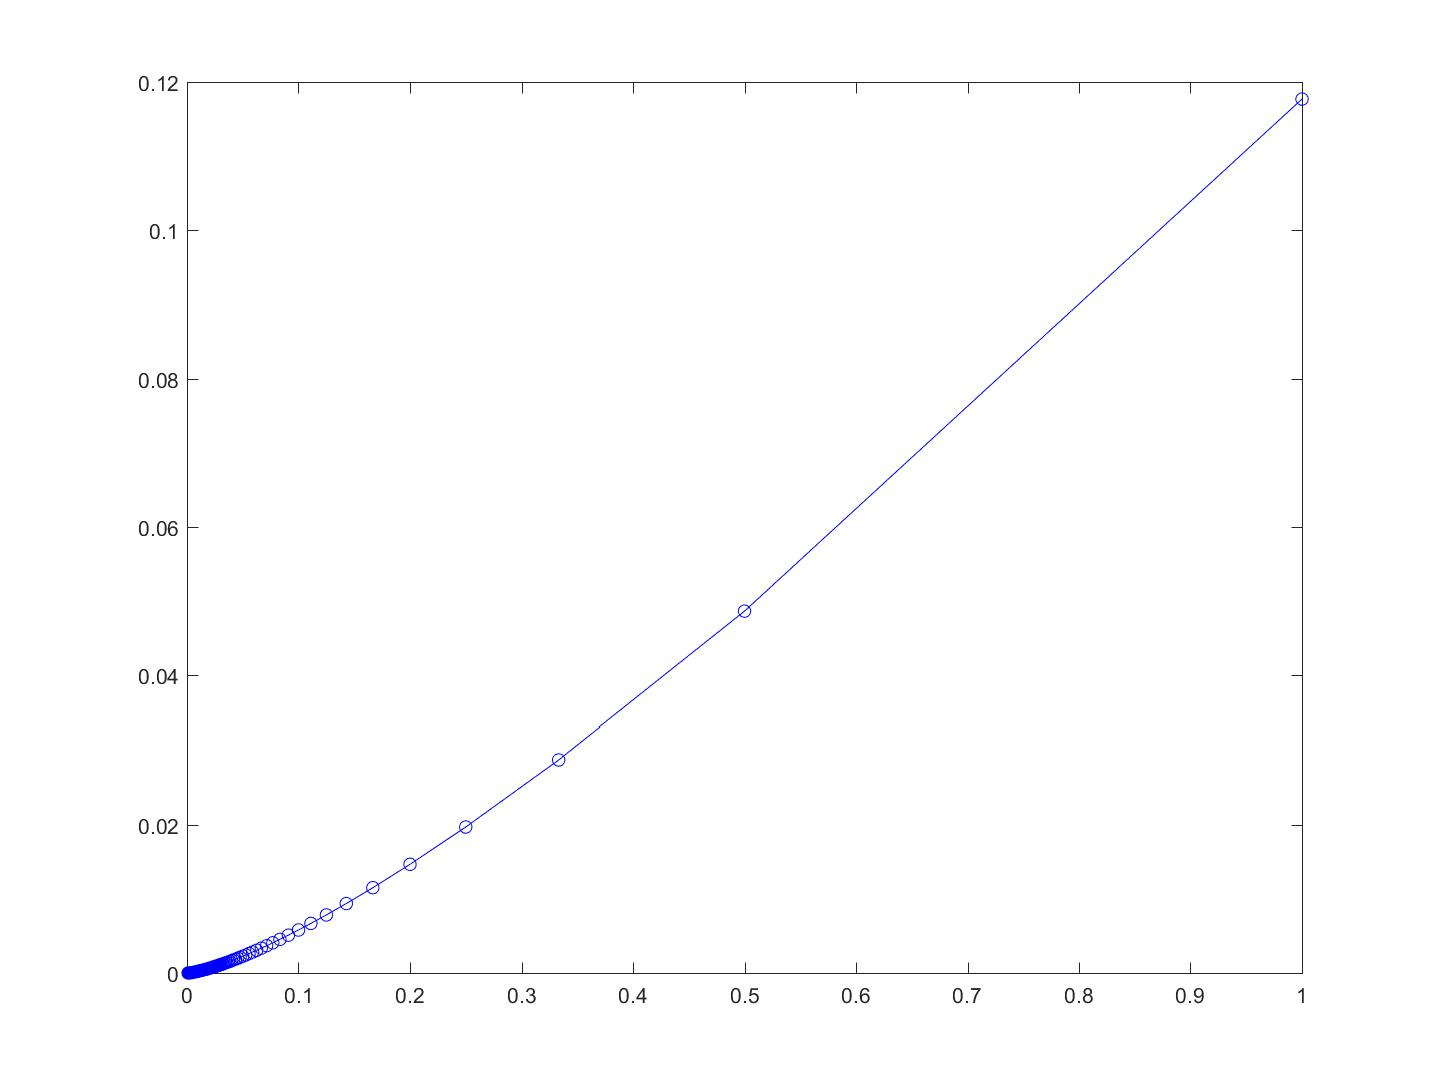
\includegraphics[height=12cm]{./Ex6c-code/simpson.jpg}
    \caption{使用复化Simpson公式的最大模误差与步长$h$的函数图像}
  \end{center}
\end{figure}
\paragraph{1.3} 比较两个公式的精度,回答问题:是否存在一个最小的$h$,使得精度不能再被改善?\\
\textbf{答:} 由上面两个公式的最大模误差与步长$h$的函数图像可以明显看出,复化Simpson公式的精度比复化梯形公式高很多,这是由于复化梯形公式的余项为
\[R_n(f) = -\frac{b - a}{12} h^2 f''(\eta), \quad \eta \in (a, b)\]
而复化Simpson公式的余项为
\[R_n(f) = -\frac{b - a}{180} \Big(\frac{h}{2}\Big)^4 f^{(4)}(\eta), \quad \eta \in (a, b)\]
根据余项公式,可知误差随$h$减小而减小,精度随$h$减小而提高,但在实际的计算中由于浮点数表示的精度有限,精度不会无限度提升.当精度已经达到机器精度时,继续减小$h$也不能再改善精度.
\begin{figure}[H]
  \begin{center}
    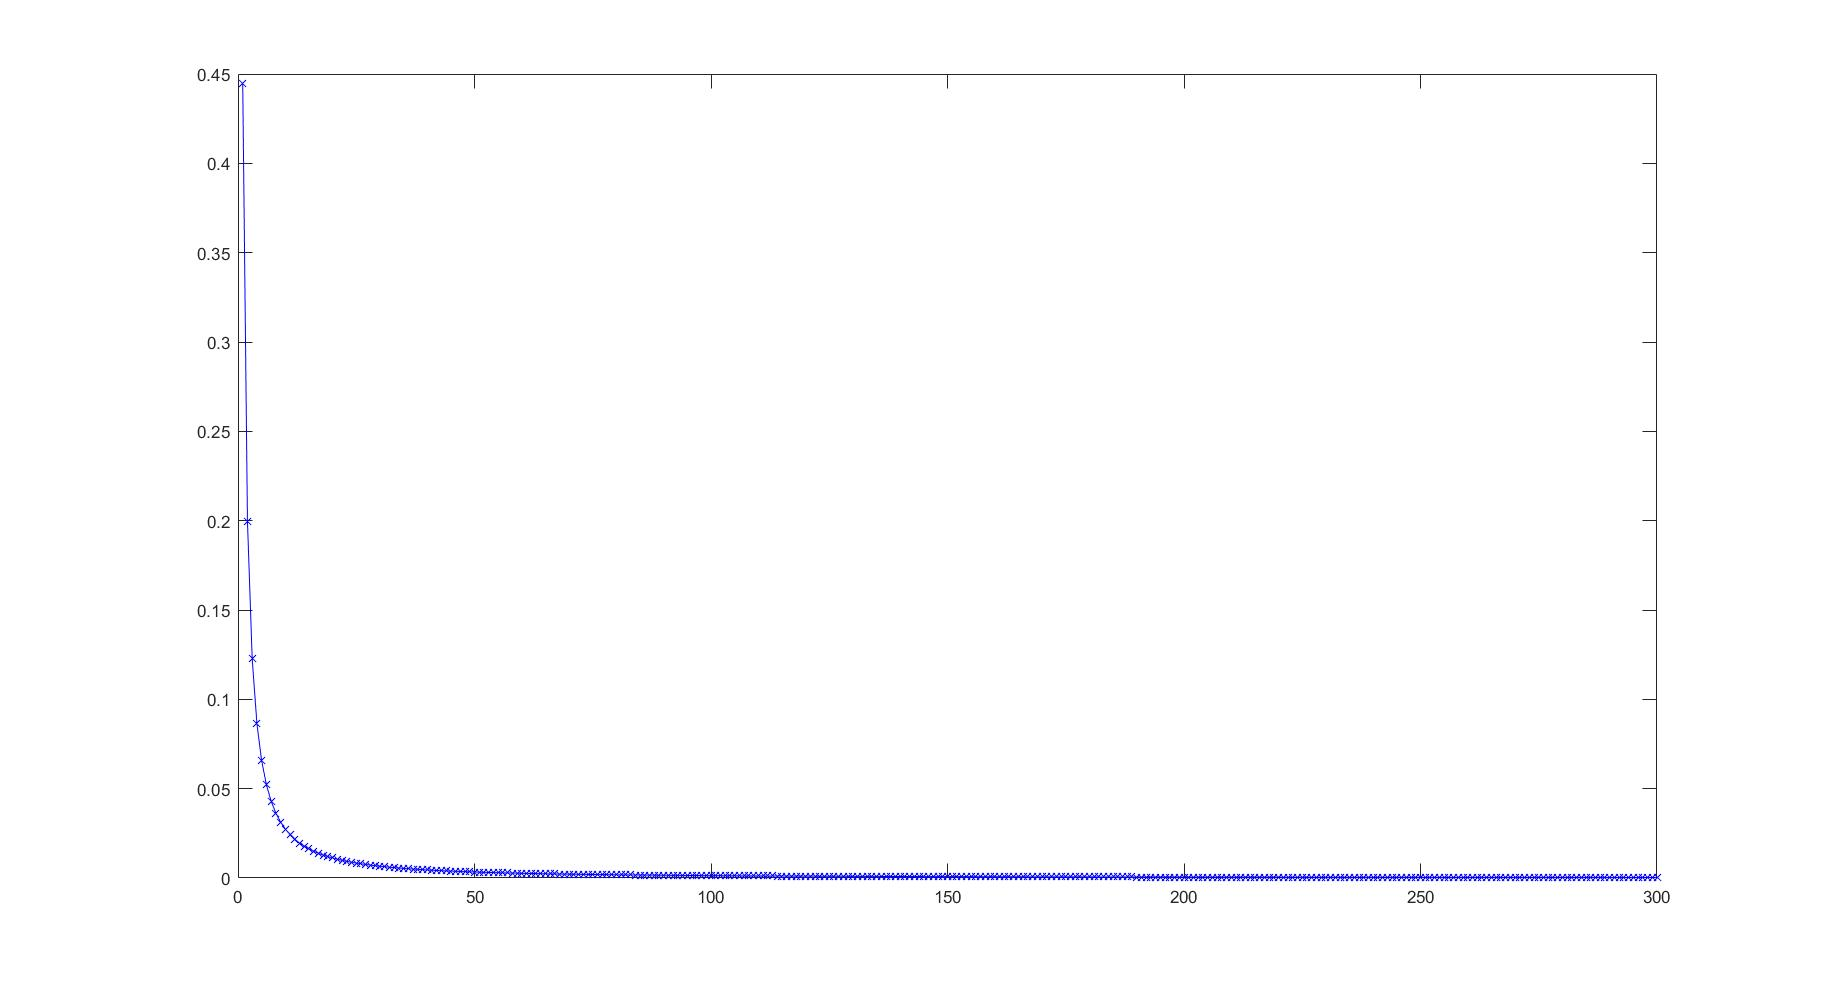
\includegraphics[height=9cm]{./Ex6c-code/delta_n.jpg}
    \caption{使用复化梯形公式的最大模误差与二分次数$n$的函数图像}
  \end{center}
\end{figure}

\section{Romberg求积方法}
\paragraph{2.1} 编写Romberg公式的函数文件,命名为Romberg.m,画出最大模误差与步长的函数图像.\\
下面实现的Romberg函数同时接受二分次数$n$和所要求的精度$eps$两个参数(其中$eps$的缺省值为0),如果二分次数达到$n$或所得结果的误差已经小于$eps$,则终止计算.
\lstinputlisting{./Ex6c-code/Romberg.m}
使用test\_room.m调用Romberg函数计算题目中的积分,并计算步长$h$取不同值时的最大模误差,画出图像如下.
\begin{figure}[H]
  \begin{center}
    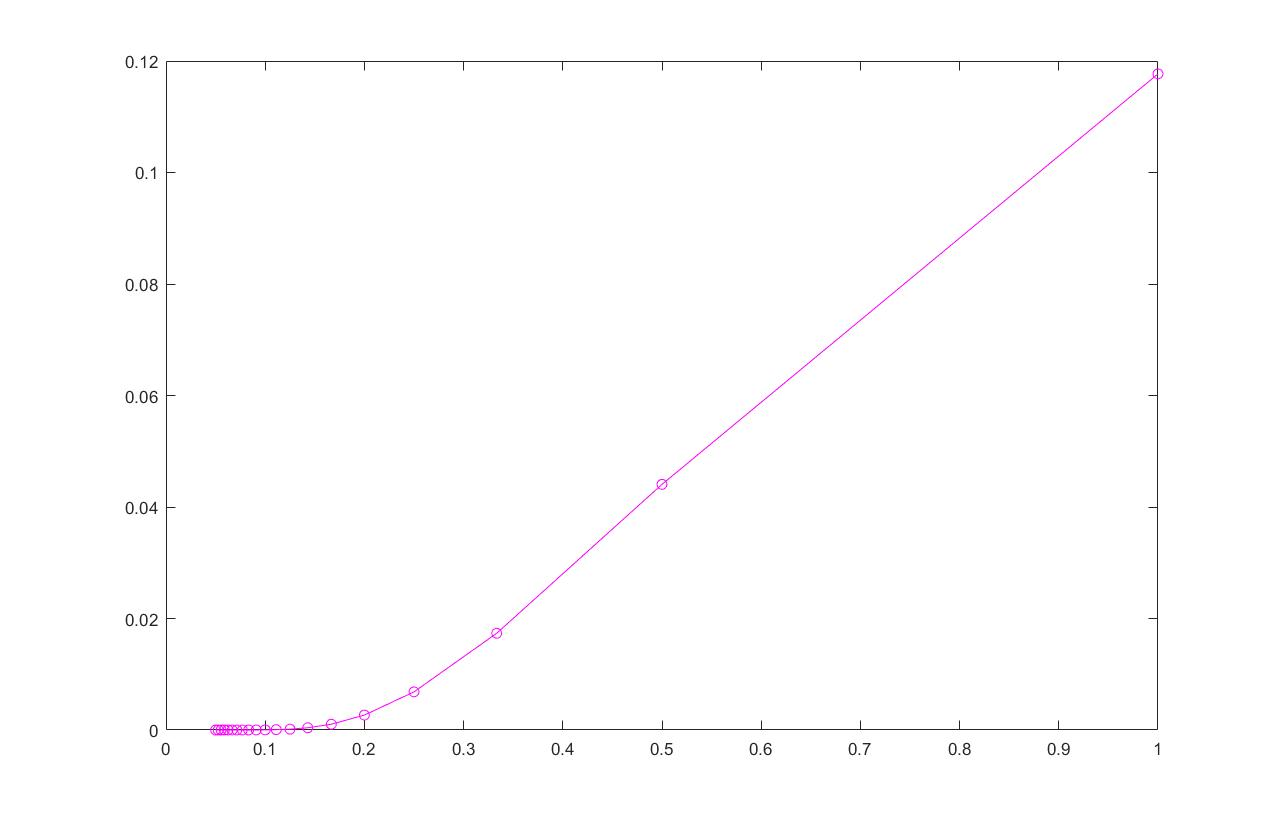
\includegraphics[height=10cm]{./Ex6c-code/romberg.jpg}
    \caption{使用Romberg公式的最大模误差与步长$h$的函数图像}
  \end{center}
\end{figure}

\section{自适应Simpson求积方法}
\paragraph{3.1} 说明如何处理二分过程中树状图扩展的问题.\\
将自适应Simpson积分实现为递归函数AdaptSimpson,在函数中计算当前区间上的积分,按照停机准则判断,若需要对当前区间进一步二分,则分别对二分得到的两个小区间调用这个递归函数,便可实现自适应Simpson积分中的树状二分扩展过程.使用时只需要对整个区间$[a, b]$调用一次AdaptSimpson函数即可.
\paragraph{3.2} 编写自适应的程序,停止准则为精度达到$10^{-4}$,程序命名为AdaptSimpson.m.\\
注:可能的话,“打印”出区间二分的详细情形.\\
下面实现的AdaptSimpson函数即为上面所述的递归函数,计算$[a, b]$区间上函数$f$的积分,要求精度为$eps$.
\lstinputlisting{./Ex6c-code/AdaptSimpson.m}
在test\_room.m中用下面的代码调用AdaptSimpson函数计算题目中的积分,得到积分结果为$-0.44444323$,最大模误差为$0.00000121$,符合精度要求.
\begin{lstlisting}
approx_I = AdaptSimpson(@ex1_fun, a, b, 10^(-4));
fprintf("%.8f %.8f\n", approx_I, abs(approx_I - I));
\end{lstlisting}
在AdaptSimpson函数中输出每次区间划分的情形,得到如下输出结果:
\begin{lstlisting}
Interval Split: [0.00000000, 1.00000000] -> [0.00000000, 0.50000000], [0.50000000, 1.00000000] 
Interval Split: [0.00000000, 0.50000000] -> [0.00000000, 0.25000000], [0.25000000, 0.50000000] 
Interval Split: [0.00000000, 0.25000000] -> [0.00000000, 0.12500000], [0.12500000, 0.25000000] 
Interval Split: [0.00000000, 0.12500000] -> [0.00000000, 0.06250000], [0.06250000, 0.12500000] 
Interval Split: [0.00000000, 0.06250000] -> [0.00000000, 0.03125000], [0.03125000, 0.06250000] 
Interval Split: [0.00000000, 0.03125000] -> [0.00000000, 0.01562500], [0.01562500, 0.03125000] 
Interval Split: [0.00000000, 0.01562500] -> [0.00000000, 0.00781250], [0.00781250, 0.01562500] 
Interval Split: [0.00000000, 0.00781250] -> [0.00000000, 0.00390625], [0.00390625, 0.00781250] 
Interval Split: [0.00000000, 0.00390625] -> [0.00000000, 0.00195313], [0.00195313, 0.00390625] 
Interval Split: [0.00000000, 0.00195313] -> [0.00000000, 0.00097656], [0.00097656, 0.00195313] 
Interval Split: [0.00000000, 0.00097656] -> [0.00000000, 0.00048828], [0.00048828, 0.00097656] 
Interval Split: [0.00000000, 0.00048828] -> [0.00000000, 0.00024414], [0.00024414, 0.00048828] 
Interval Split: [0.00000000, 0.00024414] -> [0.00000000, 0.00012207], [0.00012207, 0.00024414] 
Interval Split: [0.00000000, 0.00012207] -> [0.00000000, 0.00006104], [0.00006104, 0.00012207] 
Interval Split: [0.00000000, 0.00006104] -> [0.00000000, 0.00003052], [0.00003052, 0.00006104]
\end{lstlisting}

\end{document}